\chapter{Complément orthogonal, applications}
\label{chapter:Fr_23-orthogcomp}

\section{Complément orthogonal}
Dans le chapitre pr\'ec\'edent, nous avons vu une propriété importante de la projection orthogonale : en notant $\proj_W(\vv)$ la projection d'un vecteur $\vv\in V$ orthogonalement sur un sous-espace $W\subseteq V$, on a que le vecteur $\vv-\proj_W(\vv)$ est {\it orthogonal à tout vecteur de $W$}. Ceci suggère la définition suivante.



\begin{definition}
Soit $U$ un sous-espace de $\R^n$.  Le \defn{complément orthogonal} de $U$
est l'ensemble noté $U^\perp$ et défini par :
$$
U^\perp = \set{ \vv \in \R^n \st\uu \cdot \vv = 0 \textrm{\; pour tout $\uu\in U$}}.
$$
Voir une illustration dans la Figure \ref{figure:Uperp}. (Remarque : le complément orthogonal de $U$ est unique.)
\end{definition}

\begin{figure}
\begin{center}
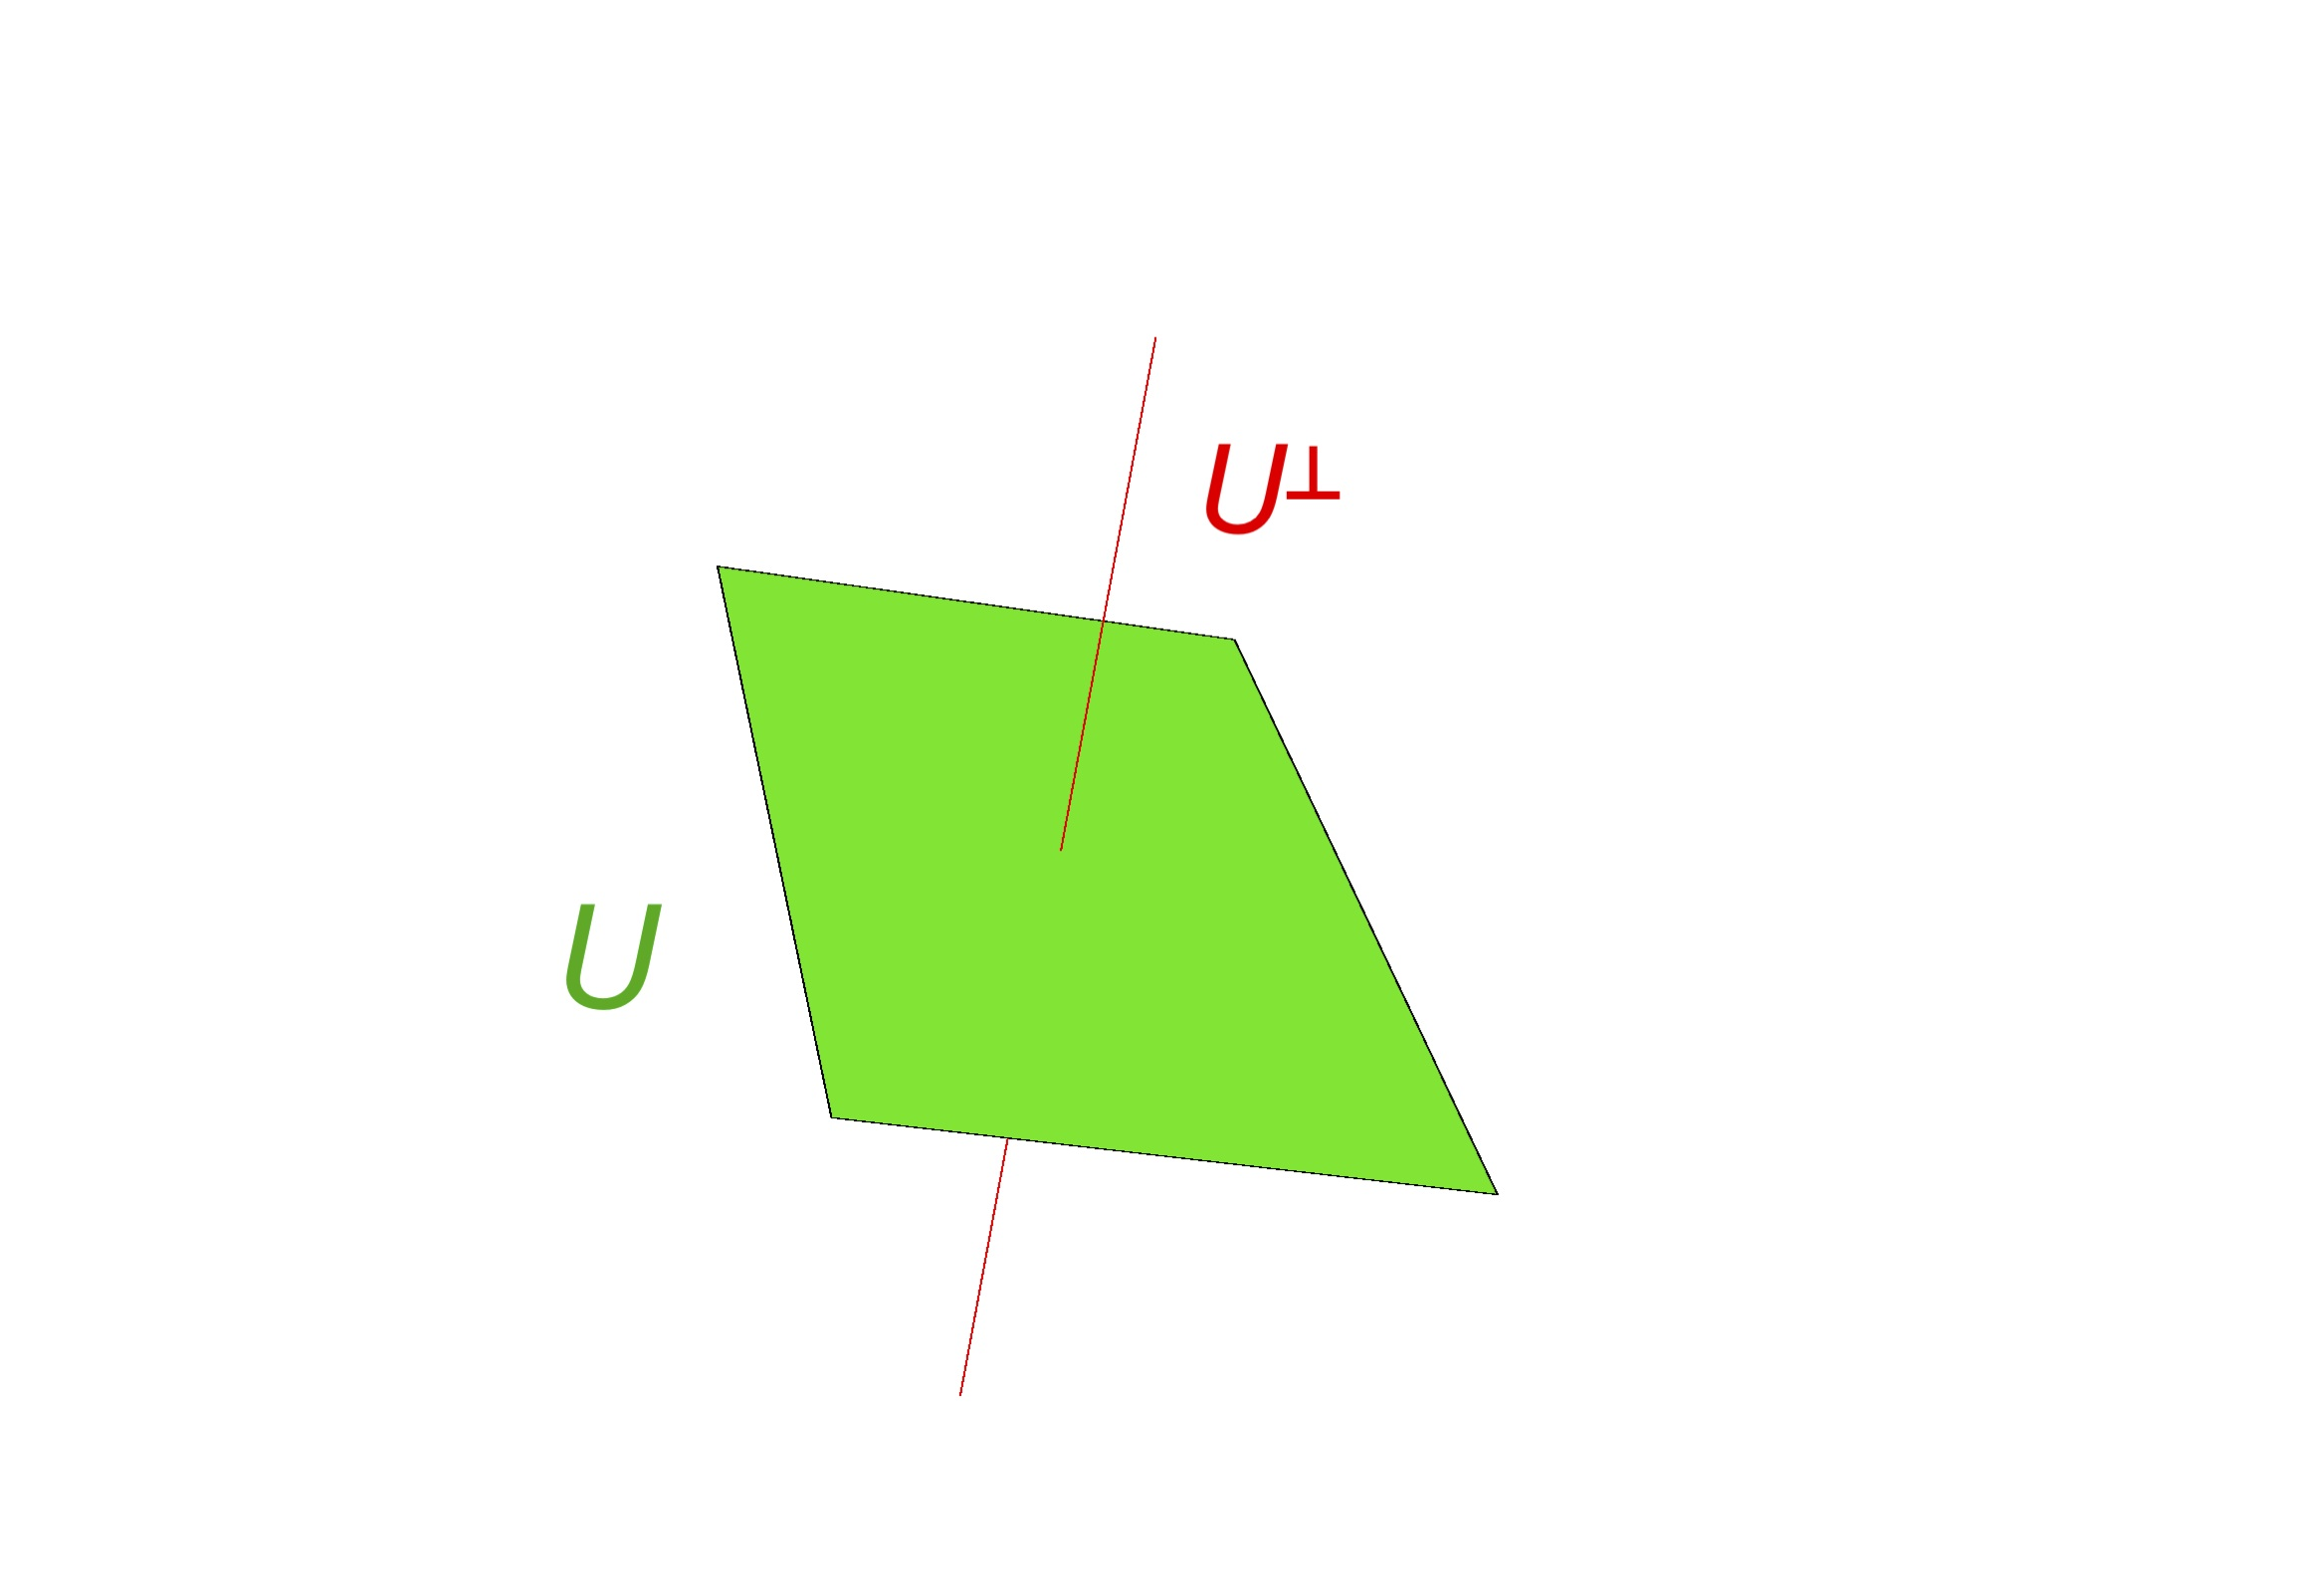
\includegraphics[scale=.5] {Uperp.jpg}~
\end{center} 
\vglue-.5cm
\caption{Le plan $U$ et son complément orthogonal.}\label{figure:Uperp}
\end{figure}

\begin{myexample}


Soit le sous-espace $U = \spn\{ (1,0,3), (0,1,2)\}$. Nous savons que $U$ est un plan passant par l'origine, et il est défini par le vecteur normal $(1,0,3) \times (0,1,2)=(-3, -2, 1)$. (On a calculé le produit vectorielle, cf. les chapitres précédents.) 

Un vecteur $\vv\in\R^3$ est donc orthogonal à $U$ si et seulement s'il est parallèle à $(-3, -2, 1)$. Ainsi,  

$$U^\perp=\sp{(-3, -2, 1)}.$$ 

En d'autres termes, l'ensemble $U^\perp$ est aussi un sous-espace : c'est la droite passant par l'origine et de vecteur directeur $(-3, -2, 1)$.
\end{myexample}


\begin{myexample}
Soit $U$ le sous-espace de $\R^4$ défini par $U=\sp{(1,-1,0,-1)} $. 

Rappel : un vecteur est $\vv\in\R^4$ orthogonal à tout vecteur de $U$ si et seulement si $\vv$ est orthogonal aux vecteurs d'une base de $U$ (voir la preuve du Théorème~\ref{orthogproj} page \pageref{orthogproj}). En d'autres termes, un vecteur $\vv=(x,y,z,w)\in\R^4$ appartient à $U^\perp$ si et seulement si 
$$(x,y,z,w)\cdot (1,-1,0,-1)=0.$$ Mais le membre de gauche est égal à $ x - y - w$, donc on en déduit l'expression de $U^\perp$ :
$$U^\perp = \set{(x,y,z,w)\in \R^4\st x - y - w=0}\,.
$$
(Vous reconnaîtrez peut-être le sous-espace comme $W$ qu'on avait étudié \`a la page~\pageref{example:GS} parmi les deux derniers exemples du chapitre précédent.)
\end{myexample}

Qu'en est-il de $W^\perp$ si $W=U^\perp$ de l'exemple pr\'ec\'edent ?\medskip

\begin{myexample}
Soit $W=\set{(x,y,z,w)\in \R^4\st x - y - w = 0}$.

Nous savons que qu'un vecteur $\vv \in \R^4$ appartient à $W^\perp$ si et seulement si $\vv$ est orthogonal à tout vecteur d'une base de $W$. Nous connaissons plusieurs bases de $W$ : par exemple, à partir de l'exemple \`a la page~\pageref{Wagain}, nous savons que l'ensemble suivant est une base de $W$ :
$$ \set{\vv_1=(1,0,0,1), \vv_2=(1,1,1,0), \vv_3=(2,1,-1,1)}\,.$$ 
Donc nous devons juste trouver tous les $\vv$ de $\R^4$ tels que les trois équations suivantes sont vérifiées :
\begin{align*}
\notag \vv_1\cdot \vv&=0,\\
\vv_2\cdot \vv&=0, \tag{$\ast$}\label{eqn:aaa}\\
\notag \vv_3\cdot \vv&=0\,.
  \end{align*}

Nous avons déjà vu ce genre de chose auparavant ! Vous souvenez-vous de la Remarque~\ref{NullperpRow} à la page \pageref{NullperpRow} ? Elle disait en partie que pour une matrice $A$ donnée, un vecteur $\vv$ est orthogonal à chaque ligne de $A$ si et seulement si $\vv$ appartient à $\ker(A)$.

Or, en prenant la matrice $  A=\scriptsize  \bmatrix ~&\vv_1&~\\&\vv_2 \\&\vv_3\endbmatrix$ définie par blocs de lignes, on voit que les trois équations \eqref{eqn:aaa} sont satisfaites si et seulement si $\vv$ est orthogonal aux lignes de $A$, et donc par ce qu'on a dit ci-dessus, c'est équivalent à chercher $\vv$ dans le noyau $\ker(A)$. Ceci nous dit que $W^\perp = ker(A)$.
Calculons donc $\ker(A)$ :
$$W^\perp = \ker(A)=\ker \bmatrix  1&0&0&1\\1&1&1&0\\2&1&-1&1\endbmatrix =\ker\bmatrix  1 & 0 & 0 & 1 \\
 0 & 1 & 0 & -1 \\
 0 & 0 & 1 & 0 \\\endbmatrix=\set{(-s,s,0,s)\st s\in \R}\,.$$
Donc le singleton $\set{(-1,1,0,1)}$ est une base de $\ker(A)= W^\perp$, et on trouve que $W^\perp = U$.
\end{myexample}

Au final, avec les deux exemples précédents, nous avons les relations $W=U^\perp$ et $W^\perp = U$. Donc nous aboutissons à l'égalité suivantes :
$$(U^\perp)^\perp=U~!$$  
Mais cette égalité est-elle toujours vraie pour tout sous-espace $U$ de $\R^n$ ?
OUI, c'est bien le cas, et d'autres r\'esultats sont également vrais :

\begin{theorem}[Propriétés du complément orthogonal]\index{propriétés du complément orthogonal}\label{orthogcompprop}
Soit $U$ un sous-espace de $\R^n$.  Alors :
\begin{enumerate}[(1)]
\item $U^\perp$ est un sous-espace de $\R^n$;
\item $(U^\perp)^\perp = U$;
\item et $\dim(U) + \dim(U^\perp) = n$.
\end{enumerate}
Lorsque deux sous-espaces $U$ et $V$ satisfont l'égalité $U = V^\perp$ (ou de manière équivalente
$V = U^\perp$), alors on dit qu'ils sont des \defn{compléments orthogonaux l'un de l'autre}.
\end{theorem}

\begin{proof}
\begin{enumerate}[(1)]
	\item On applique le test des sous-espaces.  Rappelons la définition de $U^\perp$ :
$$
U^\perp = \{ \vv \in \R^n \mid \uu \cdot \vv = 0 \textrm{\; pour tout $\uu\in U$}\,.
 \}
$$
(a) Puisque le vecteur nul $\zero$ est orthogonal à tous les vecteurs de $U$ (il est même orthogonal
à tout vecteur de $\R^n$ !), on a bien $\zero \in U^\perp$. 

(b) Supposons que $\vv, \ww\in U^\perp$.  Alors $\uu \cdot \vv= 0$ et $\uu \cdot \ww =0$ pour tout $\uu\in U$.  Est-ce que $\vv + \ww \in U^\perp$?  On calcule :
$$
\uu \cdot (\vv + \ww) = \uu \cdot \vv + \uu \cdot \ww = 0 + 0 = 0.
$$
Donc, c'est bon, on a bien la stabilité par addition : $\vv + \ww \in U^\perp$. 

(c) Supposons que $\vv \in U^\perp$ et que $k\in \R$.  Par définition, on a $\uu \cdot \vv = 0$ pour tout $\uu\in U$.
L\`a encore, on calcule :
$$
\uu \cdot (k\vv) = k\uu \cdot \vv = k (0) = 0\,,
$$
donc on a bien la stabilité par multiplication par un scalaire : $k\vv \in U^\perp$. 

D'o\`u $U^\perp$ satisfait les trois points $(a), (b), (c)$ du test des sous-espaces, et c'est donc bien un sous-espace de $\R^n$.


	\item[(3)] Soit $\{\uu_1,\ldots, \uu_k\}$ une base de $U$.
Considérez la matrice $ A=\scriptsize  \bmatrix ~&\uu_1&~\\&\vdots \\&\uu_k\endbmatrix$ dont les bloc de lignes sont les vecteurs de cette base.
Alors l'ensemble de tous les vecteurs $\vv$ orthogonaux à $U$
est exactement l'ensemble des vecteurs $\vv$ tels que $A\vv = \zero$
(en utilisant l'argument de l'exemple ci-dessus).  Donc $U^\perp = \ker(A)$.
Or, par le Théorème du rang on a :
$$
\dim(\row(A)) + \dim(\ker(A)) = n\,,
$$
et le terme de gauche est égal à $\dim(U) + \dim(U^\perp)$. D'où l'égalité voulue.

	\item[(2)] Posons $V = U^\perp$. C'est un sous-espace par (1)
et sa dimension est $n - \dim(U)$ par (3).   Nous voulons conclure que $U = V^\perp$.  Puisque tout vecteur de $U$ est en effet orthogonal à tout vecteur de $V$, il est vrai que $U \subseteq V^\perp$.  De plus, par (3), on a que:
$$\dim(V^\perp) = n- \dim(V) = n-(n-\dim(U)) = \dim(U)\,.$$  
En résumé, l'ensemble $U$ est un sous-espace de $V^\perp$ 
qui a la même dimension que $V^\perp$, donc il est nécessairement \'egal \`a $V^\perp$.
(On a utilisé le théorème qui dit que si un sous-espace n'est pas l'espace entier, alors il
doit avoir une dimension strictement inf\'erieure \`a celle du plus grand espace).
\end{enumerate}
\end{proof}

\begin{myprob}
Soit $A$ une matrice quelconque.  Montrez que $\row(A)$ et $\ker(A)$ sont toujours compléments orthogonaux l'un de l'autre. Montrez le même résultat pour $\im(A)$ et $\ker(A^T)$.  

\begin{mysol}

C'est une reprise de notre exemple pr\'ec\'edent dans un cadre plus général.
Supposons que $A$ soit une matrice $m \times n$.
Rappelons que $\ker(A)=\set{\xx \in \R^n\st A \xx=\zero}$.
Par définition de la multiplication matricielle, l'égalité $A\xx=\zero$ revient à
dire que le produit scalaire de chaque ligne de $A$ avec $\xx$ est égal à 0, donc $$\ker(A)=\set{\xx \in \R^n \st \xx \text{ est orthogonal à chaque ligne de } A}\,.$$ 

Puisque les lignes de $A$ engendrent $\row(A)$, on a donc que $\xx \in \ker(A)$ si et seulement si $\xx$ est orthogonal à tout vecteur de $\row(A)$. Ainsi $\ker(A)=\row(A)^\perp$ comme requis.

Pour voir que $\ker(A^T)=\im(A)^\perp$, utilisez l'égalité $\ker(A)=\row(A)^\perp$ et substituez $A$ par $A^\perp$ pour obtenir $\ker(A^T)=\row(A^T)^\perp$. Concluez alors en utilisant le fait que $\im(A)=\row(A^T)$.
\end{mysol}
\end{myprob}






\section{Lien avec la projection orthogonale}

Utilisons ce que nous savons sur les compléments orthogonaux pour trouver une autre façon de calculer la projection orthogonale. Ne vous laissez pas décourager par le premier exemple. Il est facile -- nous aurions pu le faire au lycée, mais la méthode que nous utiliserons sera très différente et conduira à la nouvelle méthode de calcul de la projection orthogonale.

\bigskip
\begin{myprob}
Trouvez la projection de $\bb = (1,2,3)$ sur le sous-espace $U$ 
engendr\'e par $\{ (1,1,1)\}$.

\begin{mysol}
On cherche un vecteur $\vv \in U$ tel que $\bb-\vv \in U^\perp$.
Pensez à $U = \im(A)$, où $A =\scriptsize \mat{1\\1\\1}$.
Alors par l'exercice précédent $U^\perp = \ker(A^T)$.  

Comme $U = \im(A)$, tout vecteur $\vv$ de $U$ peut 
s'écrire $\vv=A\xx$ pour un certain $\xx\in\R^1$.
Dire que $\bb-\vv = \bb-A\xx$ est dans $U^\perp = \ker(A^T)$
signifie que 
$$
A^T(\bb-A\xx) = \zero
$$
ou encore
$$
 A^T\bb = A^TA\xx.
$$
Mais $A^TA = (1,1,1)\cdot (1,1,1) = 3$ et $A^T\bb = \mat{1 & 1 & 1}\scriptsize\mat{1\\2\\3} = 6$. Donc $\xx = 2\in\R^1$, et notre r\'eponse est :
$$
\proj_U(\bb) = \vv = A\xx = \mat{2\\2\\2}\,.
$$
Notez que cette réponse coïncide bien avec ce qu'on aurait obtenu en utilisant notre formule d'avant :
$$
\proj_{\mathbf{(1,1,1)}}((1,2,3)) = \frac{(1,2,3)\cdot (1,1,1)}{\|(1,1,1)\|^2} \mat{1\\1\\1} = \mat{2\\2\\2}\,,
$$
mais nous avons choisi de faire une autre méthode qui sera utile pour la suite.
\end{mysol}\end{myprob}

En fait, nous venons de trouver un deuxième moyen de calculer la projection sur
{\it tout} sous-espace de $\R^n$.

\begin{theorem}[Deuxième méthode pour calculer la projection]\index{calcul de la projection -- deuxième méthode}
Soit $U$ un sous-espace de $\R^n$ et soit $A$ une matrice telle que
$\im(A) = U$.  Alors $\proj_U(\bb)$ est le vecteur $A\xx$, 
où $\xx$ est une solution quelconque du système
$$
A^TA \xx = A^T \bb.
$$
\end{theorem}

Pour le prouver, il suffit d'appliquer l'argument de l'exemple ci-dessus.
Et puisque nous savons que $\proj_U(\bb)$ existe toujours, notez que le système  
$A^TA \xx = A^T \bb$ sera {\it toujours} compatible !

\section{Application : approximation des solutions d'un système incompatible}

\begin{corollary}[Meilleure approximation d'une solution]\index{meilleure approximation d'une solution d'un système incompatible}
Supposons que le système $A\xx = \bb$ soit incompatible.  Alors la
\defn{meilleure approximation} d'une solution de ce système est
tout vecteur $\zz$ qui résout
$$
A^TA \zz = A^T \bb\,.
$$
(On dit qu'un vecteur $\zz$ est la \emph{meilleure approximation} s'il minimise la fonction $\Vert A\zz - \bb \Vert$.)
\end{corollary}

\begin{proof}
Minimiser $\Vert A\zz - \bb \Vert$ sur tout $\zz \in \R^n$ 
signifie trouver le vecteur dans $\im(A)$ le plus proche de $\bb$ car $\im(A)$ est exactement l'ensemble des vecteurs de la forme $A\zz$.
Donc, pour un vecteur minimisant $\zz$, le vecteur image $A\zz$ est nécessairement $\proj_{\im(A)}(\bb)$. L'égalité voulue découle ensuite du théorème précédent.
\end{proof}

\begin{myprob}
Trouvez la meilleure approximation d'une solution pour le système incompatible $A\xx = \bb$, où $\bb = (1,2,1,2)$ et
$$
A = \mat{1 & 0 & 1 \\ 0 & 1 & 0 \\ 0 & 0 & 1\\ 0 & 0 & 0}\,.
$$
 
\begin{mysol}
Appliquons ce corollaire.
On a d'une part :
$$
A^T A = \mat{1 & 0 & 0 & 0\\ 0 & 1 & 0 & 0 \\ 1 & 0 & 1 & 0}
\mat{1 & 0 & 1 \\ 0 & 1 & 0 \\ 0 & 0 & 1\\ 0 & 0 & 0}
=\mat{1 & 0 & 1\\ 0 & 1 & 0 \\ 1 & 0 & 2}
$$
et d'autre part :
$$
A^T\bb = \mat{1 & 0 & 0 & 0\\ 0 & 1 & 0 & 0 \\ 1 & 0 & 1 & 0}\mat{1\\2\\1\\2} = \mat{1 \\ 2\\ 2}\,.
$$
On doit donc r\'esoudre
$$
\mat{1 & 0 & 1\\ 0 & 1 & 0 \\ 1 & 0 & 2}\mat{x\\y\\z} = \mat{1 \\ 2\\ 2},
$$
ce que nous ferons en r\'eduisant par rapport aux lignes
$$
\mat{1 & 0 & 1 &|& 1\\ 0 & 1 & 0 &|& 2\\ 1 & 0 & 2&|& 2}
\sim 
\mat{
1 & 0 & 0 &|& 0\\ 
0 & 1 & 0 &|& 2\\ 
0 & 0 & 1&|& 1}\,.
$$
On a alors la solution unique $(0,2,1)$.  Comme c'est la première fois, vérifions que le vecteur
$$
\xx=\mat{0\\2\\1}
$$
donne bien la meilleure approximation d'une solution au
système $A \xx = \bb$. On a
$$
\mat{1 & 0 & 1 \\ 0 & 1 & 0 \\ 0 & 0 & 1\\ 0 & 0 & 0}\mat{0\\2\\1} = \mat{1\\2\\1\\0}
$$
ce qui n'est pas tout à fait $\bb$ mais en est assez proche.
Pour être vraiment convaincu que c'est la meilleure approximation, considérez n'importe quelle autre solution $\vv=(x,y,z)$ 
puis calculez 
$$
A\vv = \mat{x+z\\ y\\ z\\ 0}\,.
$$
Donc 
$$
\Vert (1,2,1,2) - (x+z, y, z, 0) \Vert^2 = (1-(x+z))^2 + (2-y)^2 + (1-z)^2 + 2^2\,,
$$
ce qui est $\geq 2^2 = 4$ car les trois premiers termes sont $\geq0$ dans le terme de droite. Or, on remarque que notre solution $(0, 2, 1)$ permet d'atteindre cette borne minimale $4$. Donc on ne peut pas faire strictement mieux que notre solution, ce qui montre bien que notre solution est la meilleure approximation d'une solution.
\end{mysol}\end{myprob}




\section[Application : méthode des moindres carrés]{Application: méthode des moindres carrés}\label{leastsquares}

\begin{myprob} Vous êtes en train de faire une expérience et vous recueillez les données suivantes:

\begin{center}
\begin{tabular}{|c|c|}
\hline x & y \\
\hline 
-2 & 18 \\
-1 &  8.1 \\
0 & 3.8\\
1 & 3.1\\
2 & 6.1\\
\hline
\end{tabular}
\end{center}
En les plaçant sur un graphique, vous voyez que ces points de données ne sont pas exactement sur une parabole, mais vous pensez que c'est dû à une erreur expérimentale et qu'il faudrait quand même trouver la parabole la plus proche de ces points. Quelle est donc la fonction quadratique la plus ajustée par rapport \`a ces points ?

\begin{mysol} 
À première vue, il ne s'agit pas d'un problème linéaire.
Reformulons-le donc comme un problème d'algèbre linéaire pour pouvoir le résoudre avec nos outils !

Nous voulons trouver un polynôme de degr\'e 2 (une fonction quadratique) de la forme suivante :
$$
y = a + bx + cx^2\,,
$$
de sorte que lorsque l'on substitue une des valeurs $x$ ci-dessus, on obtient une valeur \ \og \ proche\ \fg\ 
de la valeur $y$ que nous avons mesurée.

En fait, voici ce qu'on veut faire : trouver les coefficients $a,b,c$ solutions du système linéaire suivant (du moins à des erreurs près) :
\begin{align*}
a + b(-2) + c(-2)^2 &= 18\\
a + b(-1) + c(-1)^2 &= 8.1\\
a + b(0) + c(0)^2 &= 3.8\\
a + b(1) + c(1)^2 &= 3.1\\
a+ b(2) + c(2)^2 &= 6.1\,.
\end{align*}
C'est l'équation matricielle
$
A\xx = \bb\,,
$
o\`u
$$
A = \mat{1 & -2 & 4\\ 1 & -1 & 1\\ 1 & 0 & 0 \\ 1 &  1& 1\\ 1 & 2 & 4}, \quad\quad \xx=\mat{a\\b\\c} \qquad\textrm{et }\qquad  \bb = \mat{18\\8.1\\3.8\\3.1\\6.1}\,.
$$
Le problème, c'est que ce système est incompatible... (vérifiez-le !)
Donc, nous savons d'après ce qui précède que nous devrions résoudre plutôt le système 
$$
A^TA \xx = A^T\bb\,,
$$
o\`u
$$
A^TA = \mat{5&0&10\\0&10&0\\10&0&34}
\qquad
\textrm{et} 
\qquad 
A^T\bb = \mat{39.1\\-28.8\\107.6}\,,
$$
ce qui donne (après réduction par rapport aux lignes, et peut-être l'aide d'une calculatrice)
$$
\xx = \mat{3.62\\-2.88\\2.1} = \mat{a\\b\\c}.
$$
Ceci signifie que la quadratique qu'on cherche est
$$
y = (3.62) - (2.88)\,x + (2.1)\, x^2\,.
$$
(Vous auriez besoin d'un calculateur graphique pour vérifier si c'est vraiment le meilleur ajustement possible de parabole par rapport aux données).
\end{mysol}\end{myprob}

Dans quel sens était-ce la «~meilleure réponse~» ?  Nous avons minimisé la distance entre
$A\xx$ et $\bb$.  Rappelons que si $\xx = (a,b,c)$, alors $A\xx$ donne
la liste des valeurs de $y=a+bx+cx^2$ quand \'evalu\'e aux valeurs de $x$ données dans la deuxième colonne de $A$. Notons $y_{-2}, y_{-1}, y_0, y_1, y_2$ ces valeurs de $y$ qu'on obtient ainsi.
 Par ailleurs, le vecteur $\bb$
donne les valeurs réellement mesurées dans l'expérience ; notons $y'_{-2}, y'_{-1}, y'_0, y'_1, y'_2$ ces valeurs expérimentales.
Nous avons donc minimisé
$$
\Vert A\xx - \bb \Vert^2 = (y_{-2}-y'_{-2})^2 + (y_{-1}-y'_{-1})^2 + (y_0-y'_0)^2 + (y_1-y'_1)^2 + (y_2-y'_2)^2\,;
$$
c'est-à-dire qu'on a trouvé ce qu'on appelle le \defn{meilleur ajustement des moindres carrés} : c'est  la courbe qui minimise la somme des carrés
des différences entre les valeurs de $y$ théorique et expérimentales.

\standout{Les \emph{moindres carrés} est une technique standard pour ajuster une courbe polynomiale à des données expérimentales.}

\paragraph{Résumé de la méthode:}

\begin{enumerate}
\item Données expérimentales : points de coordonnées $(x_i,y_i)$, pour $i=1,\cdots, n$.
\item Objectif : trouver le meilleur polynôme $p$ de degré $m$ correspondant à ces données expérimentales :
$$
p(x) = a_0 + a_1x+ \cdots + a_mx^m\,.
$$
\item Poser $$
A = \mat{1 & x_1 & x_1^2 & \cdots & x_1^m \\
1 & x_2 & x_2^2 & \cdots & x_2^m \\
\ldots & \ldots & \ldots & \ddots & \ldots \\
1 & x_n & x_n^2 & \cdots & x_n^m}\,,
\quad\quad
\xx = \mat{a_0\\a_1\\\vdots\\a_m}
\qquad \textrm{et} \qquad
\bb = \mat{y_1\\y_2 \\ \ldots \\ y_n}\,.
$$
\item R\'esoudre $(A^TA) \xx = (A^T\bb)$.
\item La solution $\xx$ vous donnera la courbe la plus proche des données expérimentales \emph{au sens des moindres carrés}.
\end{enumerate}



